\chapter{Performing a Local Experiment on Single Board Heater System}\label{sercomm}
This chapter explains the procedure to use Single Board Heater System locally with Scilab i.e. when you are physically accessing SBHS using your computer. An open loop experiment, step test is used for demonstrating this procedure. The process however remains the same for performing any other experiment explained in this document, unless specified otherwise. 
\section*{Hardware and Software Requirements}\label{umlauts}
For working with the Single Board Heater system, following components are required:

\begin{enumerate}
\item SBHS with USB cable and power cable.
\item PC/Laptop with Scilab software installed. Scilab can be downloaded from:\\ {\tt http://www.scilab.org}
\item FTDI Virtual Com Port driver corresponding to the OS on your PC. Linux users do not need this. The driver can be downloaded from:\\
{\tt http://www.ftdichip.com/Drivers/VCP.htm}

\end{enumerate}


\section{Using SBHS on a Windows OS}
\label{win_procedure}
This section deals with the procedure to use SBHS on a Windows Operating System. The Operating System used for this document is Windows 7, 32-bit OS. If you are using some other Operating System or the steps explained in section \ref{driver} are not sufficient to understand, refer to the official document available on the main ftdi website at {\tt www.ftdichip.com}. On the left hand side panel, click on 'Drivers'. In the drop-down menu, choose 'VCP Drivers'. Then on the web page page, click on 'Installation Guides' link. Choose the required OS document. We would now begin with the procedure.
\subsection{Installing Drivers and Configuring COM Port}\label{driver}
After powering ON the SBHS and plugging in the USB cable to the PC (check the jumper settings on the board are set to USB communication) for the very first time, the {\tt Welcome to Found New Hardware Wizard} dialog box will pop up. Select the option {\tt Install from a list or specific location}. Choose {\tt Search for best driver in these locations}. Check the box {\tt Include this location in the search}. Click on {\tt Browse}. Specify the path where the driver is copied as explained earlier (item no.3) and install the driver by clicking {\tt Next}. Once the wizard has successfully installed the driver, the SBHS is ready for use. Please note that this procedure should be repeated twice.

Now, the communication port number assigned to the computer port to which the Single Board Heater System is connected, via an RS232 or USB cable should be identified. For identifying this port number, right click on {\tt My Computer} and click on { \tt Properties}. Then, select the { \tt Hardware} tab and click on { \tt Device Manager}. The list of hardware devices will be displayed. Locate the Ports(COM \& LPT) option and click on it. The various communication ports used by the computer will be displayed. If the SBHS is connected via RS232 cable, then look for Communications Port(COM1) else look for USB Serial Port. For RS232 connection, the port number mostly remains COM1. For USB connection it may change to some other number. Note the appropriate COM number. This process is illustrated in figure \ref{com_number}
\begin{figure}
\centering
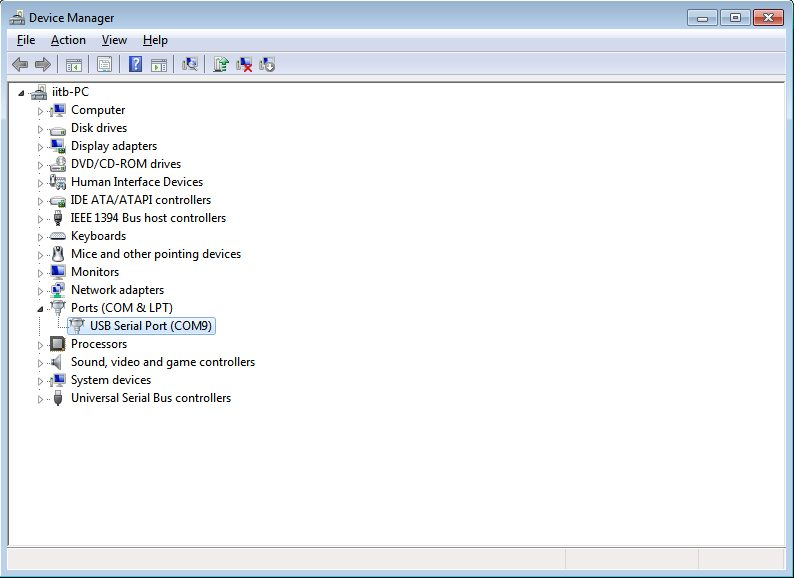
\includegraphics[width=0.7\linewidth]{using-sbhs/COM.jpg}
\caption{Checking Communication Port number}
\label{com_number}
\end{figure}

Sometimes the COM port number associated with the USB port after connecting a USB cable may be greater than 9. Since the serial tool box can handle only single digit port number (upto 9), it is necessary to change this COM port number. Following is the procedure to change the COM port number.
Double click on the name of the particular port. Click on { \tt Port Settings} tab and then click on { \tt Advanced}. In the COM port number drop-down menu, choose the port number to any other number less than 10. This procedure is illustrated in figure \ref{com_change}. After following the procedure the COM port number can be verified as described earlier.

Scilab must be installed on your computer. We recommend the use of scilab-5.3.3. This is because all the codes are created and tested using scilab-5.3.3. These codes may very well work in higher versions of scilab but one cannot use the same codes back again in scilab-5.3.3. This is because a software is always backward compatible, never forward compatible. Scilab for windows or linux can be downloaded from {\tt scilab.org}. However, if scilab-5.3.3 for your OS is not available on {\tt scilab.org} then one can download it from {\tt sbhs.os-hardware.in/downloads}. Installation of scilab on windows is very straight-forward. After you download the .exe file one has to double click on it and proceed with the instructions given by the installer. All default options will work. However, note that scilab on windows requires internet connection during installation.
\begin{figure}
\centering
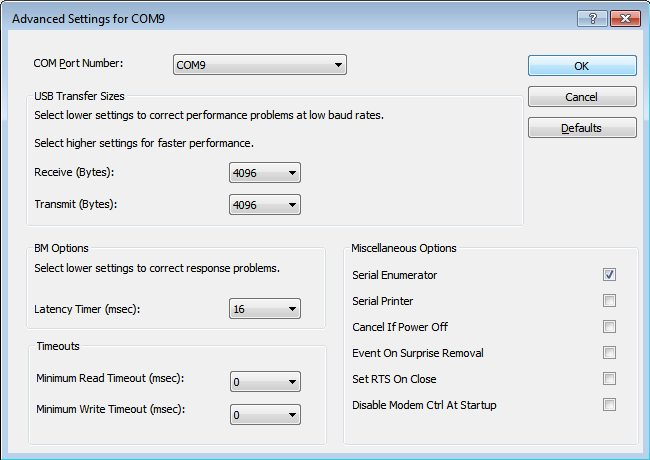
\includegraphics[width=0.7\linewidth]{using-sbhs/port2.jpg}
\caption{Changing Com port number}
\label{com_change}
\end{figure}
\subsection{Steps to Perform a Local Experiment}\label{local-steps}
\label{scilab_sbhs}
Go to {\tt sbhs.os-hardware.in/downloads}. Let us take a look at the downloads page. There are two versions of the scilab code. One which can be used with SBHS locally i.e. when you are physically accessing SBHS using your computer and another to be used for accessing SBHS virtually. This section expects you to download the local version. On extracting the file that you will download, you will get a folder {\tt local}. This folder will contain many folders named after the experiment. You will also find a directory named {\tt common-files}. We are going to use the folder named {\tt Step\_test}.
\begin{enumerate}
\item Launch Scilab from start menu or double click the Scilab icon on the desktop (if any). Before executing any scripts which are dependent on other files or scripts, one needs to change the working directory of Scilab. This will set the directory path in Scilab from where the other necessary files should be loaded.  To change the directory, click on file menu and then choose "Change directory". This can also be performed by typing {\tt cd<space>folder path}. Change the directory to the folder  {\tt Step\_test}. There is another quicker way to make sure you are in the required working directory. Open the experiment folder. Double click on the scilab file you want to execute. Doing so will automatically launch scilab and also automatically change the working directory. To know your working directory at any time, execute the command {\tt pwd} in the scilab console. 
\item Next, we have to load the content of {\tt common-files} directory. Notice that this directory is just outside the {\tt Step\_test} directory. The  {\tt common-files} directory has several functions written in .sci files. These functions are required for executing any experiment. To load these functions type \\{\tt getd<space>folder path}. The {\tt folder path} argument will be the complete path to {\tt common-files} directory. Since this directory is just outside our {\tt Step\_test} directory, the command can be modified to \\{\tt getd<space>..\textbackslash common\_files\ } So now we have all functions loaded. 
\item Next we have to load the serial communication toolbox. For doing so we have to execute the {\tt loader.sce} file present in the {\tt common-files} directory. To do so execute the command \\{\tt exec<space>..\textbackslash common\_files\textbackslash loader.sce} or\\ {\tt exec<space>folder path\textbackslash loader.sce}. 
\item Next, click on {\ttfamily editor} from the menu bar to open the Scilab editor or simply type {\ttfamily editor} on the Scilab console and open the file {\ttfamily ser\_init.sce}. Change the value of the variable {\tt port2} to the COM number identified for the connected SBHS. For example, one may enter {\tt 'COM5'} as the value for port2. Notice that there is no space between COM and 5 and COM5 is in single quotes.  Keep all other parameters untouched. Execute this .sce file by clicking on the execute button available on the menu bar of scilab editor window. The message {\tt COM Port Opened} is displayed on successful implementation. If there are any errors, reconnecting the USB cable and/or restarting Scilab may help.
\item Next we have to load the function for the step test experiment. This function is written in {\tt step\_test.sci} file. Since we do not have to make any changes in this file we can directly execute it from scilab console without opening it. Run the command {\tt exec<space>step\_test.sci} in scilab console.  The results are illustrated in figure \ref{loader}. 

\item Next, type {\ttfamily Xcos} on the Scilab console or click on { \ttfamily Applications} and select {\ttfamily Xcos} to open Xcos environment. Load the {\ttfamily step\_test.xcos} file from the { \ttfamily File} menu. The Xcos interface is shown in figure \ref{Xcosintr}. The block parameters can be set by double clicking on the block. To run the code click on {\ttfamily Simulation} menu and click on {\ttfamily Start}. After executing the code in Xcos successfully the plots as shown in figure \ref{plots} will be generated. Note that the values of fan and heater given as input to the Xcos file are reflected on the board display. 
\item To stop the experiment click on the {\ttfamily Stop} option on the menu bar of the Xcos environment. 
\end{enumerate}



All of the activities mentioned above, from {\tt getd<space>..\textbackslash common\_files\ } untill starting the xcos simulation, are coded in a file named {\tt start.sce}. Executing this file will do all necessary things automatically with just click of a button. This file however assumes three things. These are

\begin{enumerate}
\item The location of {\tt common-files} directory is not changed 
\item The current working directory is correct
\item The port number mentioned in  {\ttfamily ser\_init.sce} is correct
\end{enumerate}

\begin{figure}
\centering
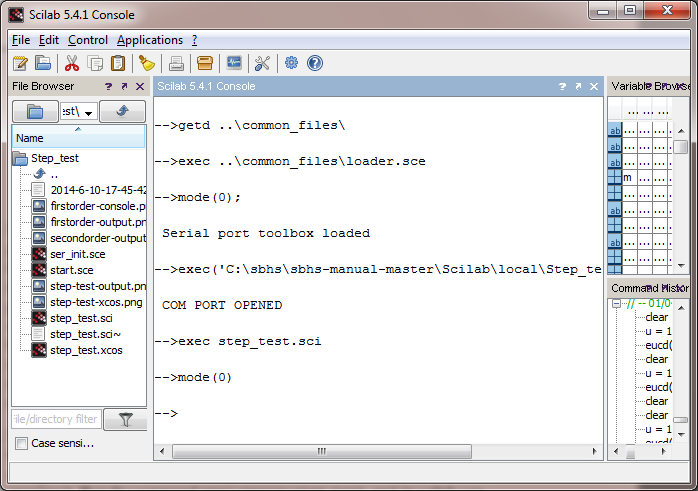
\includegraphics[width=0.7\linewidth]{using-sbhs/commands.png}
\caption{Expected responses seen on the console}
\label{loader}
\end{figure}


\begin{figure}
\centering
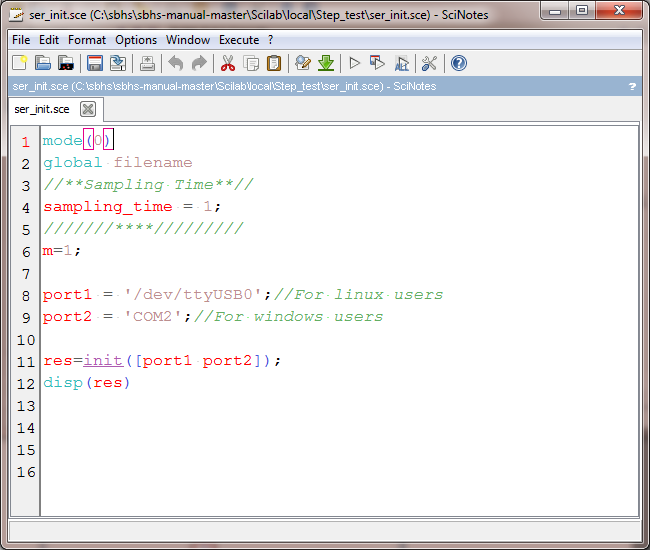
\includegraphics[width=0.7\linewidth]{using-sbhs/ser_init.png}
\caption{Executing script files}
\label{exec}
\end{figure}

\begin{figure}
\centering
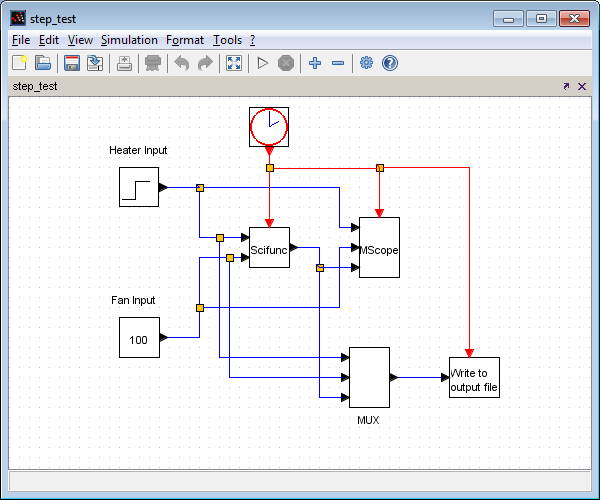
\includegraphics[width=0.7\linewidth]{using-sbhs/xcos.png}
\caption{Xcos Interface}
\label{Xcosintr}
\end{figure}

%\begin{figure}
%\centering
%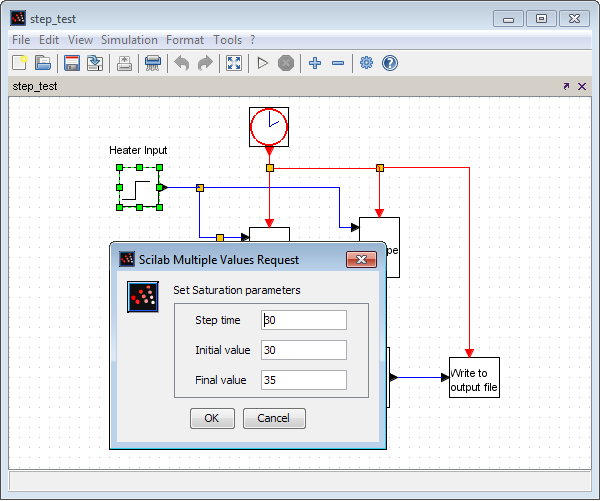
\includegraphics[width=0.7\linewidth]{using-sbhs/xcos_block.png}
%\caption{Setting Block Parameters}
%\label{blk_parameters}
%\end{figure}


\begin{figure}
\centering
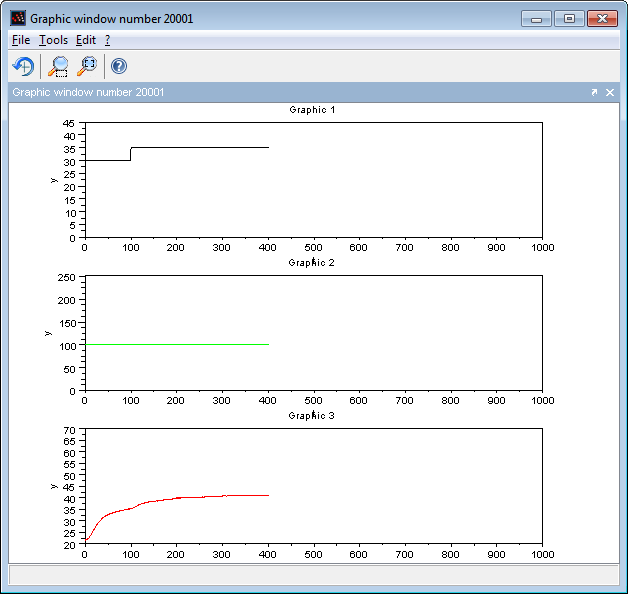
\includegraphics[width=0.7\linewidth]{using-sbhs/plot.png}
\caption{Plot obtained after executing step\_test.xcos}
\label{plots}
\end{figure}

\section{Using Single Board Heater System on a Linux System}\label{linux-sbhs}
This section deals with the procedure to use SBHS on a Linux Operating System. The Operating System used for this document is Ubuntu 12.04.
For Linux users, the instructions given in section \ref{win_procedure} hold true with a few changes as below:

 On a linux system, Scilab-5.3.3 can be either installed from available package manager (synaptic in case of Ubuntu) or its portable version can be downloaded from {scilab.org} or {\tt http://sbhs.os-hardware.in/downloads}. If installed from a package manager then scilab can be launched by opening a terminal (Alt+Ctrl+T) and executing the command {\tt sudo scilab}. If one downloads the portable version then first the file has to unpacked. This can be done by right clicking on it and choosing {\tt Extract here}. Then one has to open the terminal and change the directory to {\tt scilab/bin}. Then the command {\tt sudo ./scilab} must be executed to launch scilab. Note that scilab must always be launched with sudo permisions to be able to communicate with the SBHS.


FTDI COM port drivers are not required for connecting the SBHS to the PC. After plugging in the USB cable to the PC, check the serial port number by typing {\tt ls /dev/ttyUSB*} on the terminal, refer Fig.\ref{lstty}.
\begin{figure}
\centering
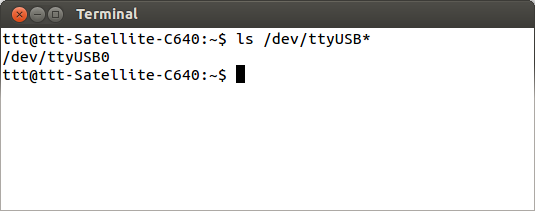
\includegraphics[width=0.7\linewidth]{using-sbhs/lstty.png}
\caption{Checking the port number in linux (1)}
\label{lstty}
\end{figure}
%\begin{figure}
%\centering
%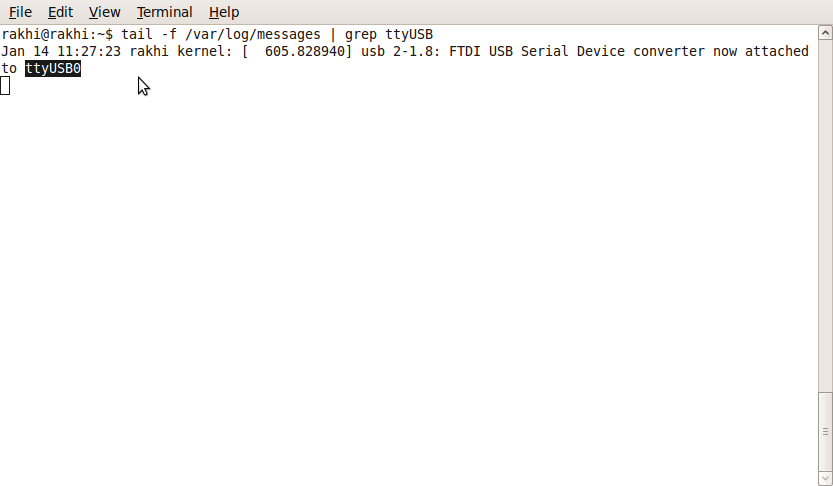
\includegraphics[width=0.7\linewidth]{using-sbhs/tailusb.png}
%\caption{Checking the port number in linux (2)}
%\label{tailusb}
%\end{figure}

Note down this number and change the value of the variable {\tt port1} inside the {ser\_init.sce} file, refer Fig.\ref{exec}. 

 Except for these changes rest all of the steps mentioned in Section \ref{local-steps} can be followed.
%\begin{figure}
%\centering
%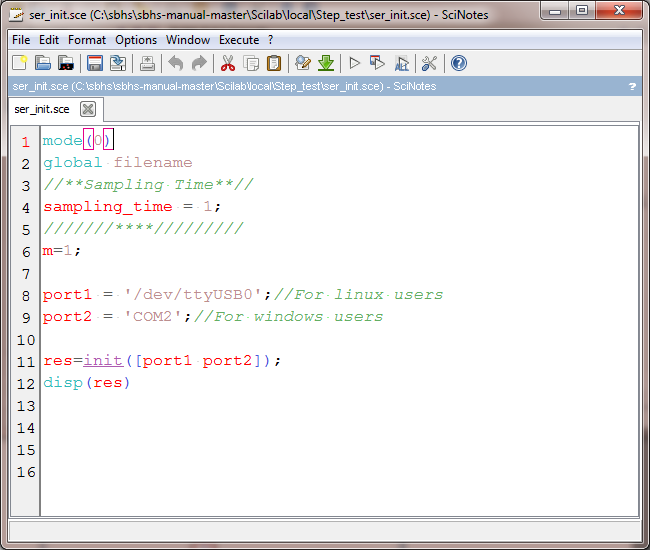
\includegraphics[width=\linewidth]{using-sbhs/ser_init.png}
%\caption{Configuring port number and other parameters}
%\label{linuxserial}
%\end{figure}


%\begin{figure}
%\centering
%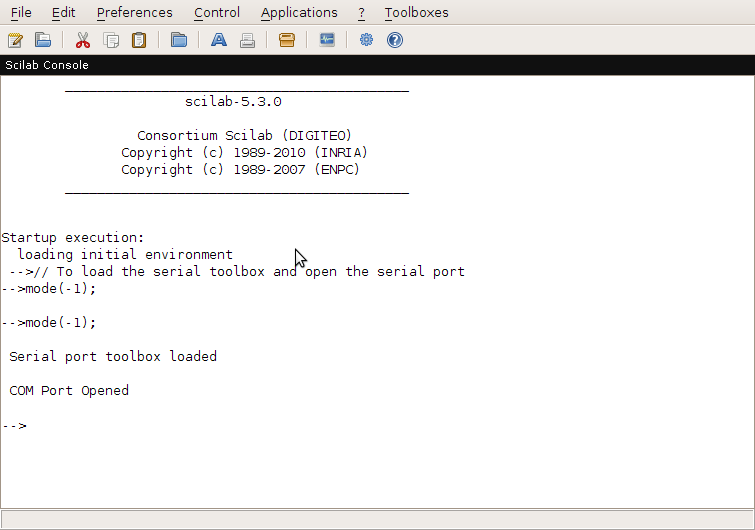
\includegraphics[width=0.7\linewidth]{using-sbhs/SSscilab.png}
%\caption{Scilab Console Message after Opening Serial Port}
%\label{console_linux}
%\end{figure}

